\documentclass[11pt]{article}

\usepackage{natbib}
\usepackage{setspace}
\usepackage[left=2.5cm,top=2.8cm,right=2.5cm,bottom=2.8cm]{geometry}
\usepackage{graphicx}
\usepackage{amsmath}
\usepackage{theorem}
\usepackage{version}
\usepackage{multirow}
\usepackage{listings}
\usepackage{hyperref}
\usepackage{algpseudocode}
\usepackage{amssymb}
\usepackage{tikz}
\usepackage{algorithm}
\usepackage{algorithmic}
\usepackage{minted}
\usepackage{graphicx}
\usetikzlibrary{arrows,arrows.meta,decorations,decorations.pathreplacing,calc,matrix}

\definecolor{Red}{rgb}{1,0,0}
\definecolor{Blue}{rgb}{0,0,1}
\definecolor{Green}{rgb}{0,1,0}
\definecolor{magenta}{rgb}{1,0,.6}
\definecolor{lightblue}{rgb}{0,.5,1}
\definecolor{lightpurple}{rgb}{.6,.4,1}
\definecolor{gold}{rgb}{.6,.5,0}
\definecolor{orange}{rgb}{1,0.4,0}
\definecolor{hotpink}{rgb}{1,0,0.5}
\definecolor{newcolor2}{rgb}{.5,.3,.5}
\definecolor{newcolor}{rgb}{0,.3,1}
\definecolor{newcolor3}{rgb}{1,0,.35}
\definecolor{darkgreen1}{rgb}{0, .35, 0}
\definecolor{darkgreen}{rgb}{0, .6, 0}
\definecolor{darkred}{rgb}{.75,0,0}
\definecolor{lightgrey}{rgb}{.7,.7,.7}

\definecolor{clemson-orange}{RGB}{234,106,32}
\definecolor{chicago-maroon}{RGB}{128,0,0}
\definecolor{northwestern-purple}{RGB}{82,0,99}
\definecolor{cornell-red}{RGB}{179,27,27}
\definecolor{sauder-green}{RGB}{171,180,0}
%\definecolor{gray}{RGB}{192,192,192}
\definecolor{lawngreen}{RGB}{0,250,154}

\setcounter{MaxMatrixCols}{10}

\onehalfspacing
\newtheorem{theorem}{Theorem}
\newtheorem{acknowledgement}{Acknowledgement}
\newtheorem{algorithm}{Algorithm}
\newtheorem{assumption}{Assumption}
\newtheorem{axiom}{Axiom}
\newtheorem{case}{Case}
\newtheorem{claim}{Claim}
\newtheorem{conclusion}{Conclusion}
\newtheorem{condition}{Condition}
\newtheorem{conjecture}{Conjecture}
\newtheorem{corollary}{Corollary}
\newtheorem{criterion}{Criterion}
\newtheorem{definition}{Definition}
\newtheorem{example}{Example}
\newtheorem{exercise}{Exercise}
\newtheorem{lemma}{Lemma}
\newtheorem{notation}{Notation}
\newtheorem{problem}{Problem}
\newtheorem{proposition}{Proposition}
{\theorembodyfont{\normalfont}
\newtheorem{remark}{Remark}
}
\newtheorem{summary}{Summary}
\newenvironment{proof}[1][Proof]{\textbf{#1.} }{\hfill \rule{0.5em}{0.5em} \bigskip}
\newenvironment{soln}[1][Soln]{\textbf{#1:} }{\hfill \rule{0.5em}{0.5em}}
\renewcommand{\cite}{\citeasnoun}
\renewcommand{\theenumii}{(\alph{enumii})}
\renewcommand{\labelenumii}{\theenumii}
\renewcommand{\theenumiii}{\roman{enumiii}}
\renewcommand{\labelenumiii}{\theenumiii.}

\usepackage[nameinlink]{cleveref}
\crefname{assumption}{Assumption}{Assumptions}
\crefname{lemma}{Lemma}{Lemmas}
\crefname{theorem}{Theorem}{Theorems}
\crefname{corollary}{Corollary}{Corollaries}
\crefname{proposition}{Proposition}{Propositions}
\crefname{claim}{Claim}{Claims}
\crefname{procedure}{Procedure}{Procedures}
\crefname{algorithm}{Algorithm}{Algorithms}
\crefname{figure}{Figure}{Figures}
\crefname{remark}{Remark}{Remarks}
\crefname{section}{Section}{Sections}
\crefname{procedure}{Procedure}{Procedures}
\crefname{example}{Example}{Examples}
\crefname{definition}{Definition}{Definitions}
\crefname{table}{Table}{Tables}
\crefname{align}{}{}
\crefname{enumi}{}{}
\crefname{conjecture}{Conjecture}{Conjectures}
\crefname{step}{Step}{Steps}
\crefname{appendix}{Appendix}{Appendices}
\crefname{footnote}{Footnote}{Footnotes}

\begin{document}


\begin{center}
    \textbf{CS 326 - Analysis of Algorithms - HW 5}\\
\end{center}


\begin{flushleft}
    \textit{Prof. M. Grigni\hfill11/18/2022 \hfill Hridansh Saraogi} \\
    \vspace{0.15cm}
    \small {Help taken from: Prof. Grigni, and Zhenke Liu}\\
    \small {Collaborators: }
\end{flushleft}


\begin{enumerate}

\item Problem 1 (push-relabel bipartite matching). \\
Suppose we want to find a maximum matching in a bipartite graph G. We first construct the flow network G' as described in Section 26.3, and then we use the generic push-relabel algorithm of Section 26.4 (instead of Ford-Fulkerson). Argue that this approach runs in O(VE) time.  Hint: show every push is saturating.
    \begin{enumerate}
        \item 
    \end{enumerate}

\pagebreak

\item Problem 2 (push-relabel gap heuristic). Exercise 26.5-5, page 760.\\
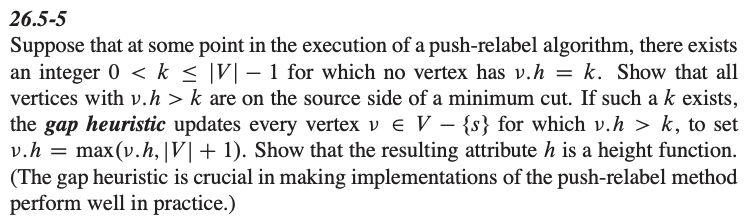
\includegraphics[scale=1]{HW5_Q2.png}
    \begin{enumerate}
        \item 
    \end{enumerate}
    
\pagebreak

\item Problem 3(HAM-CYCLE listing). Exercise 34.2-3, page 1065.\\
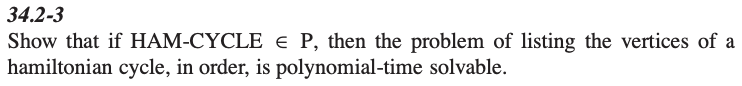
\includegraphics[scale=1]{HW5_Q3.png}
    \begin{enumerate}
        \item 
        
    \end{enumerate}

\pagebreak

\item Problem 4 ($\leq P$ is transitive). Exercise 34.3-2, page 1077. \\Hint: if p(n) and q(n) are polynomials, then so is p(q(n)).\\
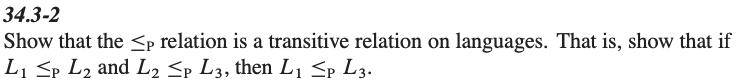
\includegraphics[scale=1]{HW5_Q4.png}
    \begin{enumerate}
        \item 
    \end{enumerate}

\pagebreak
\item Problem 5\\
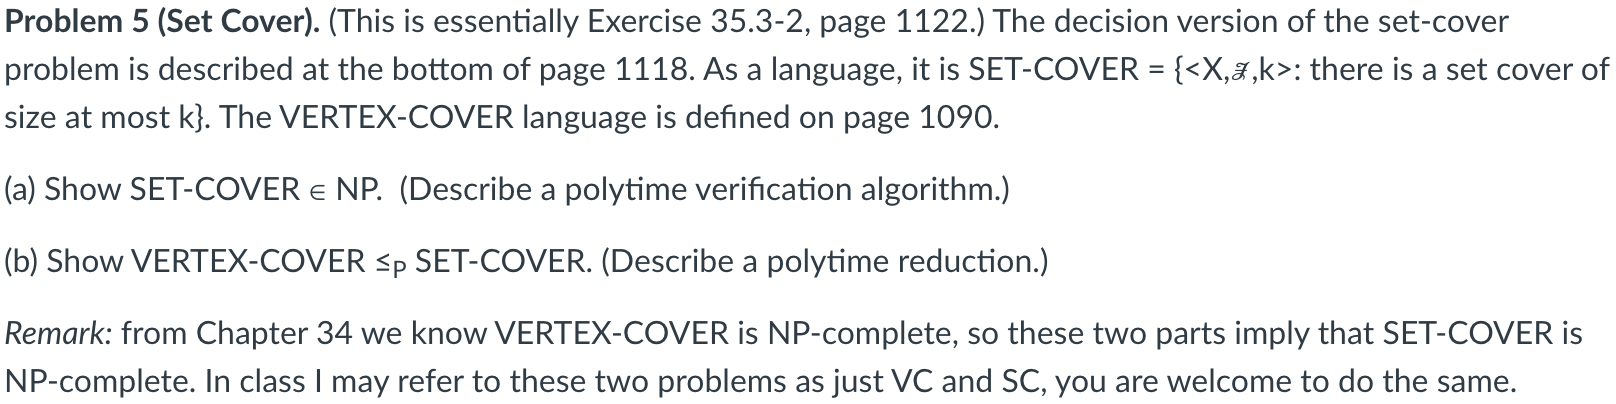
\includegraphics[scale=0.55]{HW5_Q5_1.png}\\
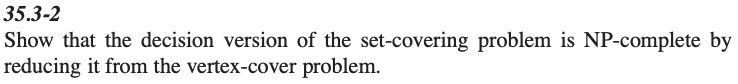
\includegraphics[scale=1]{HW5_Q5_2.png}
    \begin{enumerate}
        \item 
    
    \end{enumerate}
    
\end{enumerate}
\pagebreak


\end{document}

